\chapter{The Tokai to Kamioka Experiment}
\label{chap:detectors}

The Tokai to Kamioka (T2K) experiment was proposed and designed in the early to mid 2000s with the intent of observing electron neutrino appearance ($\nu_\mu \rightarrow \nu_e$) transition, alongside precision measurements of muon neutrino disappearance ($\nu_\mu \rightarrow \nu_\mu$)\cite{t2k_loi,t2k_prop}. Previous long baseline experiments K2K\cite{k2k_obs} in Japan and MINOS\cite{minos_obs} in the US had pioneered measuring muon neutrino disappearance in a neutrino ``beam'' over long distances, confirming the 2005 Super-Kamiokande results for $\Delta m^2$ and $\sin^2 \theta_{23}$ from atmospheric neutrinos\cite{sk_2005}. However, neither were able to confirm electron neutrino appearance with significance.

The precision measurement era took off when the independent short baseline reactor anti electron-neutrino experiments Daya Bay\cite{daya_bay_disc} and RENO\cite{reno_disc} observed in 2012, followed by indications from Double Chooz\cite{chooz_disc} in 2013, anti electron-neutrino disappearance ($\bar{\nu}_e \rightarrow \bar{\nu}_e$) with a larger $\sin^2 2\theta_{13}$ than anticipated. T2K independently observed electron neutrino appearance\cite{t2k_disc} in 2014 with an even larger mixing angle when fixing $\Delta m^2$ and $\sin^2 \theta_{23}$ to global best-fit values, the neutrino mass ordering to normal, and $\delta_{CP}=0$. NO$\nu$A confirmed\cite{nova_disc} the appearance measurement in 2016, also finding a large $\sin^2 \theta_{13}$ mixing amplitude.

The large $\sin^2 \theta_{13}$ enabled electron neutrino appearance in neutrino beams at T2K and NO$\nu$A with relatively low number of protons-on-target (POT). The current effort in the $\nu_\mu \rightarrow \nu_e$ channel is measuring the CP violating Dirac phase, $\delta_{CP}$, which sensitivity increases further to when using recent results from Daya Bay\cite{daya_bay} and RENO\cite{reno} in the PDG\cite{pdg_2017}.

\begin{figure}[h]
	\includegraphics[width=1.0\textwidth, trim={0mm 0mm 0mm 0mm}, clip,page=1]{figures/det_chap/view/t2k_overview}
	\caption{The T2K experiment where neutrinos are created at the J-PARC complex in Tokai and the neutrino beam is characterised at the near-detectors 280 m downstream. 295 km west is the Super-Kamiokande far-detector, measuring the oscillated neutrino spectrum}
	\label{fig:t2k_overview}
\end{figure}
The neutrinos at T2K come from particle decays---primarily $K^\pm$, $\pi^\pm$ and $\mu^\pm$---after a proton beam impinges on a target at the J-PARC complex. The neutrino direction is measured by a suite of near-detectors $\sim280$ m downstream of the target and a muon monitor, providing information on the neutrino flux, directionality and interaction cross-section. One near-detector, INGRID, is a plastic scintillator and iron sandwiched detector placed on-axis, extends $\pm1\deg$ in a cross as to measure the neutrino flux and directionality, and is detailed in \autoref{sec:ingrid}. A second near-detector, ND280, sits $2.5\deg$ off-axis and is surrounded by a 0.2T magnetic field and consists of sub-detectors with multiple interaction targets and a tracker region, designed to accurately measure neutrino interactions under a similar neutrino flux to Super-Kamiokande, and is detailed in \autoref{sec:nd280}. The far detector, Super-Kamiokande, sits 295 km downstream of the target station and measures the rate of neutrino interactions on its 50,000 tonnes of purified water, detailed in \autoref{sec:sk}. A schematic of the travel is shown in \autoref{fig:t2k_overview}.

A host of other neutrino detectors---not used in this analysis---additionally sit in ``pit'' 280m from the target station with ND280 and INGRID. Examples include the liquid emulsion NINJA experiment\cite{ninja}, the water target WAGASCI\cite{wagasci} experiment and its magnetic calorimeter Baby-MIND\cite{baby_mind}. These will in the future make precision measurements of neutrino-nucleus interactions, a dominant systematic for current oscillation analyses.

\begin{figure}[h]
	\includegraphics[width=0.4\textwidth, trim={10mm 0mm 0mm 0mm}, clip,page=1]{figures/det_chap/view/image_nd.jpeg}
	\caption{The suite of near-detectors at 280 m from the target, showing ND280 and INGRID}
\end{figure}

\section{Beamline}
The J-PARC complex\cite{jparc_tdr} is used to accelerate protons to 30 GeV/c using a linear accelerator (LINAC), a rapid cycling synchrotron (RCS) and a main ring (MR) synchrotron. The MR has the ability to fast-extract into the neutrino beamline with a design power of 750 kW at 30 GeV/c, using $\sim3\times10^{14}$ protons per spill with 8 proton bunches per spill, with a spill cycle of $\sim0.5$ Hz. The spill width, which opens the trigger window at the neutrino detectors, is $\sim5 \mu$s\cite{t2k_det}.

\begin{figure}[h]
	\begin{subfigure}[t]{0.4\textwidth}
		\includegraphics[width=\textwidth, trim={0mm 0mm 0mm 0mm}, clip,page=1]{figures/det_chap/beam/beam.jpg}
		\caption{Top-view}
	\end{subfigure}
	\begin{subfigure}[t]{0.4\textwidth}
		\includegraphics[width=\textwidth, trim={0mm 18mm 0mm 0mm}, clip,page=1]{figures/det_chap/beam/sideview_beam}
		\caption{Side-view of target-dump section}
	\end{subfigure}
	\caption{The neutrino beamline for neutrinos at J-PARC}
	\label{fig:neutrino_beamline}
\end{figure}

The neutrino beamline consists of two parts and is shown in \autoref{fig:neutrino_beamline}: the primary beamline---which takes fast-extracted protons from the MR, bends them to point towards SK, and impinges them on a graphite target---and the secondary beamline---which directs the mesons from the proton-target interaction through a decay volume, finishing with a beam dump. Shortly after the target in the secondary beamline are three magnetic horns\cite{t2k_horns} which are used to deflect (focus) wrong-sign (right-sign) mesons to reduce wrong-sign and enhance right-sign neutrinos. Running the magnets at 250 kA (1.7 T) increases the neutrino flux at SK by factor $\sim17$\cite{t2k_beam}. The focused mesons pass through a $\sim96$m decay volume in which the majority of them decay. Remaining particles then strike the beam dump, which stops all mesons. Surviving high momentum muons $p_\mu > 5.0 \text{ GeV/c}$ generally pass through the beam dump, after which they are measured by muon monitors. The MUMON muon monitors (one ionisation chamber and one silicon PIN photodiode) infer the neutrino beam direction to better than 0.25 mrad and the beam intensity better than 3\%\cite{t2k_mumon,t2k_mumon2}, and is used to inform the beam simulation group.

The neutrinos come primarily from three meson decays
\begin{align*}
	\pi^+ & \rightarrow \mu^+ + \nu_\mu 		&  99.99\% 			& & K^+ & \rightarrow \mu^+ + \nu_\mu 			& 63.6\% & & K^0_L & \rightarrow \pi^- + e^+ + \nu_e 	  & 40.6\% \\
	      & \rightarrow e^+ + \nu_e 			&  10^{-4}\%		& &		& \rightarrow \pi^0 + e^+ + \nu_e 		& 5.1\%  & &	   & \rightarrow \pi^- + \mu^+ + \nu_\mu &  27.0\% \\
	      & \rightarrow \mu^+ + \nu_\mu + \gamma & 2\times 10^{-4}\%  & &		& \rightarrow \pi^0 + \mu^+ + \nu_\mu  	& 3.5\%  & &	   & & 		 &
\end{align*}

\iffalse
\begin{align*}
	\pi^+ 	& \rightarrow \mu^+ + \nu_\mu & 0.9999\\
			& \rightarrow e^+ + \nu_e 	  & 0.0001\\
	K^+   	& \rightarrow \mu^+ + \nu_\mu & 0.6355\\
			& \rightarrow \pi^0 + \mu^+ + \nu_\mu & 0.0353\\
			& \rightarrow \pi^0 + e^+ + \nu_e & 0.0507\\
	K^0_L 	& \rightarrow \pi^- + \mu^+ + \nu_\mu & 0.2704\\
			& \rightarrow \pi^- + e^+ + \nu_e & 0.4055
\end{align*}
\fi
and one leptonic decay\cite{pdg_2017}
\begin{align*}
\mu^+ \rightarrow e^+ + \bar{\nu}_\mu + \nu_e & & 100\%
\end{align*}

From the beam simulation we trace back each neutrino's parent meson, shown in \autoref{fig:flux_parents}. The $\pi$ parent is clearly dominant for both the \numu and \numubar fluxes, although the higher energy portion ($E_\nu > 3\text{ GeV}$) consists of neutrinos whose parents are $K$. The \nue and \nuebar components of the neutrino beam come primarily from the leptonic $\mu$ decay below $E_\nu = 1 \text{ GeV}$ and from $K^+$ and $K^0_L$ at $E_\nu = 2 \text{ GeV}$. Tertiary decay products, e.g. a $\pi^-$ from a $K^0_L$ decay, form large portions of the wrong-sign background.
\begin{figure}[h]
	\begin{subfigure}[t]{0.32\textwidth}
		\includegraphics[width=\textwidth, trim={0mm 0mm 0mm 0mm}, clip,page=1]{figures/det_chap/beam/numu_sk_parents}
	\end{subfigure}
	\begin{subfigure}[t]{0.32\textwidth}
		\includegraphics[width=\textwidth, trim={0mm 0mm 0mm 0mm}, clip,page=1]{figures/det_chap/beam/nue_sk_parents}
	\end{subfigure}

	\begin{subfigure}[t]{0.32\textwidth}
		\includegraphics[width=\textwidth, trim={0mm 0mm 0mm 0mm}, clip,page=1]{figures/det_chap/beam/numubar_sk_parents}
	\end{subfigure}
	\begin{subfigure}[t]{0.32\textwidth}
		\includegraphics[width=\textwidth, trim={0mm 0mm 0mm 0mm}, clip,page=1]{figures/det_chap/beam/nuebar_sk_parents}
	\end{subfigure}
	\caption{Simulated right-sign neutrino fluxes at SK, showing parents}
	\label{fig:flux_parents}
\end{figure}

The software suite for the beam simulation consists of FLUKA2011 \cite{fluka2008_1, fluka2008_2, fluka2011} which simulates hadronic interactions in target and baffle, JNUBEAM (GEANT3-based \cite{geant3}) which simulates the geometry and handles tracking, and GCALOR \cite{gcalor} which simulates hadronic re-interactions and is used as a cross-check for FLUKA\cite{t2k_beam, t2k_tn_flux}.

T2K was the first long baseline experiment to use the ``off-axis'' technique\cite{off_axis} in which the far-detector is offset from the neutrino beam center. This has two main effects: 1) it focuses the neutrino energy spectra into a narrower ``peak'' (albeit with lower overall rate than on-axis) and 2) it reduces the wrong-sign background for $\nu_e$ appearance searches. The effect, overlaid with the expected $\nu_\mu$ and $\nu_e$ neutrino flux at Super-Kamiokande, is shown in \autoref{fig:off-axis}. Since the neutrino parents are mostly from $\pi$ decay---a two-body decay---we can approximately express the neutrino energy $E_\nu$ as a function of pion-neutrino angle $\theta_{\pi,\nu}$, pion energy $E_\pi$ and mass $m_\pi$ and the muon mass $m_\mu$,
\begin{equation}
	E_\nu = \frac{m^2_\pi-m^2_\mu}{2\left( E_\pi - p_\pi \cos \theta_{\pi,\nu} \right)} 
\end{equation}

For a chosen $\cos \theta_{\pi,\nu}$, there is a maximum pion energy of $E_\pi^\text{max} = p_\pi/cos\theta_{\pi,\nu}$, giving rise to a maximum neutrino energy of
\begin{equation}
	E_\nu^\text{max} = \frac{m^2_\pi-m^2_\mu}{2E_\pi \sin^2 \theta_{\pi,\nu}} 
\end{equation}

which maximises when $\pi$ and $\nu$ are near collinear, and as $\theta$ increases the allowed neutrino energy spectrum becomes smaller. The calculated flux at SK with the neutrino oscillation probability is shown in \autoref{fig:off-axis}. The off-axis angle is chosen to maximise the flux in the primary oscillation dip at $E_\nu \sim 0.6\text{ GeV}$.
\begin{figure}[h]
	\includegraphics[width=0.4\textwidth, trim={0mm 0mm 0mm 0mm}, clip,page=1]{figures/det_chap/oaeffect_pnue_pnumu_flux}
	\caption{Effect of off-axis (OA) angle on the SK neutrino flux}
	\label{fig:off-axis}
\end{figure}

The beam power and accumulated POT has been steadily increasing from run 1 in 2010 to run 9 in 2019. Run 9 concluded with $\sim500\text{ kW}$ beam power, accumulating a total POT of $\sim3.16\times 10^{21}$\footnote{Or 5.28 mg of protons}: $1.51\times 10^{21}$ in FHC and $1.65\times 10^{21}$ in RHC modes.
\begin{figure}[h]
	\includegraphics[width=0.5\textwidth, trim= {7mm 40mm 7mm 12mm}, clip]{{figures/pow_t2k_all_toRun77full}}
	\caption{T2K protons on target and beam power for run 1-9}
	\label{fig:t2k_pot}
\end{figure}

The final simulated neutrino fluxes for run 2 to 8 at ND280 are shown in \autoref{fig:flux_1to8}. The wrong-sign background in FHC is $\sim18\%$ at the flux peak which reduces further due to the lower anti-neutrino interaction cross-section, and the \nue component is less than 1\% in the flux peak. The right-sign flux in RHC is similar to the \numu in FHC, and the majority of the contamination of \numu events in RHC mode comes from the higher \numu cross-section rather than the flux.
\begin{figure}[h]
	\begin{subfigure}[t]{0.45\textwidth}
		\includegraphics[width=\textwidth, trim={0mm 0mm 0mm 0mm}, clip,page=1]{figures/det_chap/beam/nd5_alltunedflux_run1-8_zoomed_13a}
		\caption{FHC}
	\end{subfigure}
	\begin{subfigure}[t]{0.45\textwidth}
		\includegraphics[width=\textwidth, trim={0mm 0mm 0mm 0mm}, clip,page=1]{figures/det_chap/beam/nd5_alltunedflux_run5c-7b_zoomed_antinu_13a}
		\caption{RHC}
	\end{subfigure}
	\caption{Simulated neutrino fluxes at ND280 in forward (FHC) and reverse (RHC) horn current modes}
	\label{fig:flux_1to8}
\end{figure}

\section{The Interactive Neutrino GRID}
\label{sec:ingrid}
Using the off-axis technique introduces the need for precise determination of the neutrino beam direction, as a 1 mrad uncertainty on the beam direction is followed by a 2-3\% uncertainty on the neutrino energy scale. Furthermore, sudden discontinuities of the beam or any of its subcomponents (e.g. magnetic horn, target deterioration) directly affect the neutrino flux, so measurements of the beam direction has to be done on a spill-by-spill basis.

The Interactive Neutrino GRID (INGRID) sits on-axis, 280 m downstream of the production target. It was designed to measure the neutrino beam profile to accurately predict the off-axis angle of ND280 and SK, and make inclusive neutrino cross-section measurements\cite{t2k_ingrid_xsec}. It has a cross shaped geometry and extends 10 m vertically and horizontally, shown in \autoref{fig:ingrid_det}. The cross consists of 14 identical modules and two off-axis detectors which measure the asymmetry of the neutrino beam. Each INGRID module has nine iron plates and 11 tracking scintillator plates, which are surrounded by veto planes on all sides to reject cosmic background\cite{t2k_ingrid}. Each module has a fiducial mass of iron at 7.1 tonnes, and the total cross spans roughly $1\sigma$ of the expected beam profile.
\begin{figure}[h]
	\begin{subfigure}[t]{0.47\textwidth}
		\includegraphics[width=\textwidth, trim={0mm 0mm 0mm 0mm}, clip,page=1]{figures/det_chap/ingrid/ingrid}
		\caption{Beam-view of INGRID}
	\end{subfigure}	
	\begin{subfigure}[t]{0.47\textwidth}
		\includegraphics[width=\textwidth, trim={0mm 0mm 0mm 50mm}, clip,page=1]{figures/det_chap/ingrid/ingrid_module}
		\caption{An INGRID module}
	\end{subfigure}
	\caption{The INGRID experiment}
	\label{fig:ingrid_det}
\end{figure}
INGRID also has a second type of module---the proton module\cite{t2k_ingrid_proton}---designed to measure neutrino interactions on plastic scintillator. It consists of 34 tracking plates, similar to those in the INGRID modules but with different dimensions, surrounded by the same veto planes.

INGRID has measured the neutrino event rates within 2\% of expected, with a precision on the directionality of 0.2 mrad all in agreement with expectation\cite{t2k_2015}, giving the neutrino beam center within 5 cm. The historical event rate and beam direction from MUMON and INGRID over the full time period presented in this thesis can be seen in \autoref{fig:ingrid_monitoring}. Generally, INGRID and MUMON agree within 0.2 mrad in both directions and the neutrino event rate agrees with expectation.
\begin{figure}[h]
	\includegraphics[width=0.8\textwidth, trim={0mm 0mm 0mm 0mm}, clip,page=1]{figures/det_chap/ingrid/INGRID_official_plot_until74}
	\caption{Beam characteristics measured by the INGRID and MUMON detectors over the T2K runs 1 through 8, used in this thesis}
	\label{fig:ingrid_monitoring}
\end{figure}

\section{ND280}
\label{sec:nd280}
The off-axis near detector for T2K is called ND280, and its neutrino-nucleus interaction data is the subject of this thesis. 

In contrast to INGRID, ND280 has the ability to accurately reconstruct and track particles emanating from a neutrino scattering vertex in one of its targets. It does so by surrounding its inner target sub-detector, the two FGDs, by three time projection chambers using gaseous argon, called the TPCs. This inner region is referred to as the ``tracker''. The tracker is comforted by an lead-scintillator sampling electromagnetic calorimeter (ECal) on all but the upstream side, at which a dedicated $\pi^0$ detector, the P0D, is placed. The whole detector is bathed in a 0.2 T magnetic field to enable accurate sign selection and momentum measurements coupled with the TPCs. The magnet yoke is in turn interleaved with a side muon range detector (SMRD) made of plastic scintillator strips which enable high angle tracking of $\mu$ and provides a cosmic veto. The exploded detector view is shown in \autoref{fig:nd280_expl}.
\begin{figure}[h]
	\includegraphics[width=0.6\textwidth, trim={0mm 0mm 0mm 0mm}, clip,page=1]{figures/det_chap/view/ND280Exploded-Text-Transparent-Large}
	\caption{The ND280 detector with its sub-detectors}
	\label{fig:nd280_expl}
\end{figure}

Since signal at SK is limited to the single ring $\mu$ and $e$ selections---vetoing any secondary rings from e.g. pions or high energy protons---the detector is well suited for single track cross-section measurements. It also provides information on the single $\pi^0$ cross-sections, a major background for oscillation searches looking for $\nu_\mu \rightarrow \nu_e$.

\subsection{Fine Grained Detectors}
The two fine grained detectors (FGDs)\cite{t2k_fgd} are the central targets for ND280, providing a combination of flux, energy spectrum and electron neutrino contamination at the off-axis angle of SK ($2.5\deg$). Each FGD provides 1.1 tonnes of target material and extends $186.4\times186.4\times2.02\text{ cm}$. FGD1 sits most upstream of the two and is made entirely of 15 XY planes, each of $2\times192$ bars. FGD2 provides a hybrid water-scintillator target, in which seven plastic scintillator planes identical to FGD1 but alternated with six 2.5 cm thick layers of water. The two FGDs can thereby measure interactions on both plastic (a common target in external neutrino scattering data) and $H_2 O$ (the target for SK).

The FGDs have the ability to reconstruct features of an event independent of the TPCs for contained particles. Isolated tracks are generally of lower momentum, so deposit significant energy per unit track length. Summing the total deposited energy of an isolated FGD track provides a means to distinguish protons from minimally ionising particles, such as pions. Furthermore, stopped pions may give rise to a delayed Michel $e$, which is searched for in the FGD reconstruction, for which the efficiency is above 90\%. Additionally, tracks with hits in the TPC are required to match FGD tracks to determine the interaction vertex. The FGD is also used to measure time-of-flight (ToF) of tracks to distinguish forward-going positive particles from backward-going negative particles, and vice versa.
\begin{figure}[h]
	\begin{subfigure}[t]{0.47\textwidth}
		\includegraphics[width=\textwidth, trim={0mm 0mm 0mm 0mm}, clip,page=1]{figures/det_chap/fgd/fgd_byrange}
		\caption{Track-length and particle}
	\end{subfigure}
	\begin{subfigure}[t]{0.47\textwidth}
		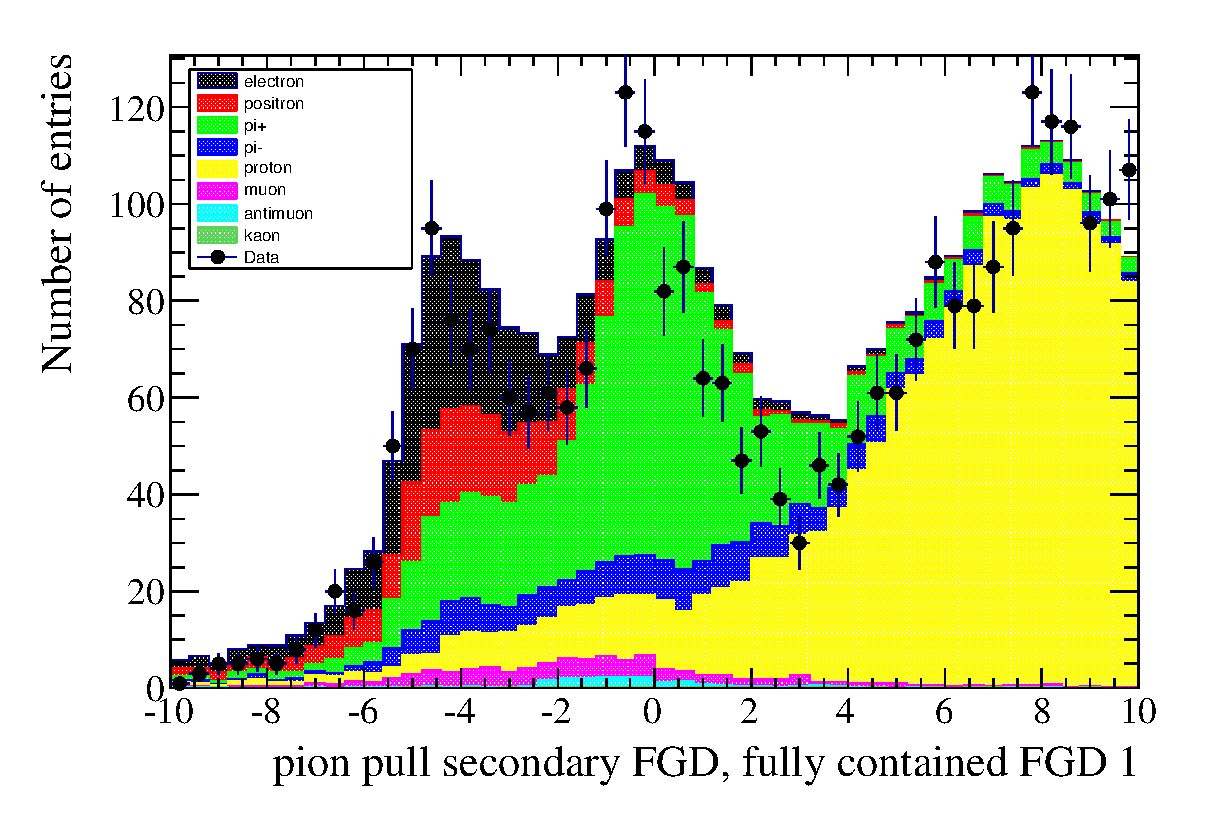
\includegraphics[width=\textwidth, trim={0mm 0mm 0mm 0mm}, clip,page=1]{figures/numu/Cuts/pull_secondarytrack_FGD_all_fullycontained}
		\caption{Particle pulls}
	\end{subfigure}	
	\caption{The FGD particle identification, using energy deposited with track length}
	\label{fig:fgd_reco}
\end{figure}

The measured track length and particle pulls for the pion hypothesis are shown in \autoref{fig:fgd_reco}. The three dominant distributions (electron/positron, pion and proton) are well separated in the pulls, agreeing relatively well with data.

Finally, the FGD is also used to for daily checks of the neutrino event rates and vertex distributions.

\subsection{Time Projection Chambers}
The three T2K time projection chambers (TPCs)\cite{t2k_tpc} provide the majority of the tracking, energy loss, particle identification and momentum measurements of the ND280 detector. All TPCs use an Ar:C$F_4$:$C_4H_10$ mixture at 95:3:2, which ionises when charged particles pass through. The ionisation electrons are drifted toward bulk micromegas detectors, amplifying the charge. The readout provides a 3D image of the paths of traversing charged particles.

Since two TPCs surround each FGD, they provide excellent tracking and multiplicity capabilities of backward and forwards-going tracks emanating in the FGD. Furthermore, neutrino interaction cross-sections are generally highest for forward-going muons and pions, and a track traversing multiple TPCs gives an improved reconstruction.

The energy loss as a function of momentum in one TPC is shown in \autoref{fig:tpc_reco} for negatively and positively charged particles. Muon/electron distinction is achieved, and MIP resolution is $7.8\pm0.2\%$. Using the particle hypotheses outlined in \autoref{sec:numu_sel}, the probability of assigning a muon to an electron hypothesis is 0.2\% for tracks below 1 GeV/c\cite{thesis_tpc}. There is also excellent ability to identify proton tracks with $p < 0.8 \text{ GeV}$.
\begin{figure}[h]
	\begin{subfigure}[t]{0.47\textwidth}
		\includegraphics[width=\textwidth, trim={0mm 0mm 0mm 0mm}, clip,page=1]{figures/numu/TPC_PID_neg}
		\caption{Negative particles}
	\end{subfigure}
	\begin{subfigure}[t]{0.47\textwidth}
		\includegraphics[width=\textwidth, trim={0mm 0mm 0mm 0mm}, clip,page=1]{figures/numu/TPC_PID_pos}
		\caption{Positive particles}
	\end{subfigure}	
	\caption{The energy loss in the TPC as a function of reconstructed momentum}
	\label{fig:tpc_reco}
\end{figure}

\subsection{Electromagnetic Calorimeter}
The ND280 E\cite{t2k_ecal}

\subsection{Pi-zero Detector}
\cite{t2k_p0d}

\subsection{Magnet}

\subsection{Side Muon Range Detector}
\cite{t2k_smrd}

\section{Super Kamiokande}
\label{sec:sk}

\cite{t2k_sk, t2k_sk2, t2k_sk3}

